\documentclass{article}

\usepackage[english]{babel}
\usepackage[utf8]{inputenc}
\usepackage{amsmath,amssymb}
\usepackage{parskip}
\usepackage{graphicx}
\usepackage{amsmath}
\usepackage{float}

% Margins
%\usepackage[top=2cm, left=2.5cm, right=2.5cm, bottom=2.5cm]{geometry}
\usepackage[margin=1in]{geometry}
% Colour table cells
\usepackage{sectsty}
\usepackage{textcomp}
\usepackage{mathtools}
\usepackage[most]{tcolorbox}

% Get larger line spacing in table
%\newcommand{\tablespace}{\\[1.25mm]}
%newcommand\Tstrut{\rule{0pt}{2.6ex}}         % = `top' strut
%\newcommand\tstrut{\rule{0pt}{2.0ex}}         % = `top' strut
%\newcommand\Bstrut{\rule[-0.9ex]{0pt}{0pt}}   % = `bottom' strut

\sectionfont{\fontsize{12}{15}\selectfont}

%%%%%%%%%%%%%%%%%
%     Title     %
%%%%%%%%%%%%%%%%%
\title{Information Visualization - Project\vspace{-0.8em}}
\author{Marian Aldescu - MoSIG DS}
\date{\today}



\begin{document}
\maketitle



\textbf{\Large{Design visualizations}}\\

\textbf{\Large{A. Global insights}}\\


\section{What is the CO$_2$ distribution over time? In which period of the year are produced the biggest CO${_2}$ emissions by Westeros missions?}

\large{\textbf{Solution 1}}\\
To answer this question, we want to show how the CO${_2}$ level evolves in time and to identify if there are periods with considerable high or low pollution. After taking a look on the dataset, I observed that the missions take place over a period of 8 years, so since the number is't not big, we can even compare how the CO${_2}$ level changes from one year to another in the same visualization.

For this question, time is not an automatic property, because the entire dataset does not evolve with time, so I will use it as a quantity(\textbf{Q}), and reserve the \textbf{X} axis for it. On the \textbf{Y} axis I will map the level of CO${_2}$ for each mission, which is also a quantity(\textbf{Q}).

On the X axis, I show the data for one year, because it would not be relevant to see all the emissions on the same axis, but overlapped or side by side. Therefore, we need to differentiate the CO${_2}$ over years, and since the years are nominal(\textbf{N}) values, I will use the retinal property(\textbf{R}) color.

According to \cite{mackinlay}, the visual mapping table will look like this:\\


\begin{table}[h!]
\begin{center}
	\begin{tabular}{|c | c | c | c || c | c | c | c | c| c| c || c|} 
		\hline
		Name & D & F & D\textquotesingle  & X & Y & Z & T & R & -& [] & CP \\ [0.5ex] 
		\hline\hline
		Time  & Q &  &  &  L &   &   &   &   &   &   &   \\ [0.5ex] 
		\hline
		CO${_2}$  & Q &  &  &  & L  &   &   &   &   &   &   \\ [0.5ex] 
		\hline
		Year  & N &  &  &  &   &   &   & C  &   &   &   \\ [0.5ex] 
		\hline
	\end{tabular}
	\caption{CO${_2}$ emissions evolution  over time}
	\label{table:1}
\end{center}
\end{table}

In Figure \ref{fig:positive_selection}, we can see a sketch of a plot using the previous visual mapping. I only drew the first 4/8 plots, normally another 4 would be overlaid. The user can choose to overlap all the plots in one by pressing \textbf{OVERLAP} button. This would help to better compare 2 or more years. Since in total, there are 8 years, the guideline for mapping of Bertin\cite{bertin} is not respected, because he recommends to use maximum 7 colors in order for the eye to do a proper selection of the elements in the visualization, but this issue can be solved  by choosing which year to keep in the plot, by checking the boxes in the right side. By pressing \textbf{EXPAND}, the visualization will be restored to the previous state.

\begin{figure}[H]
	\centering
	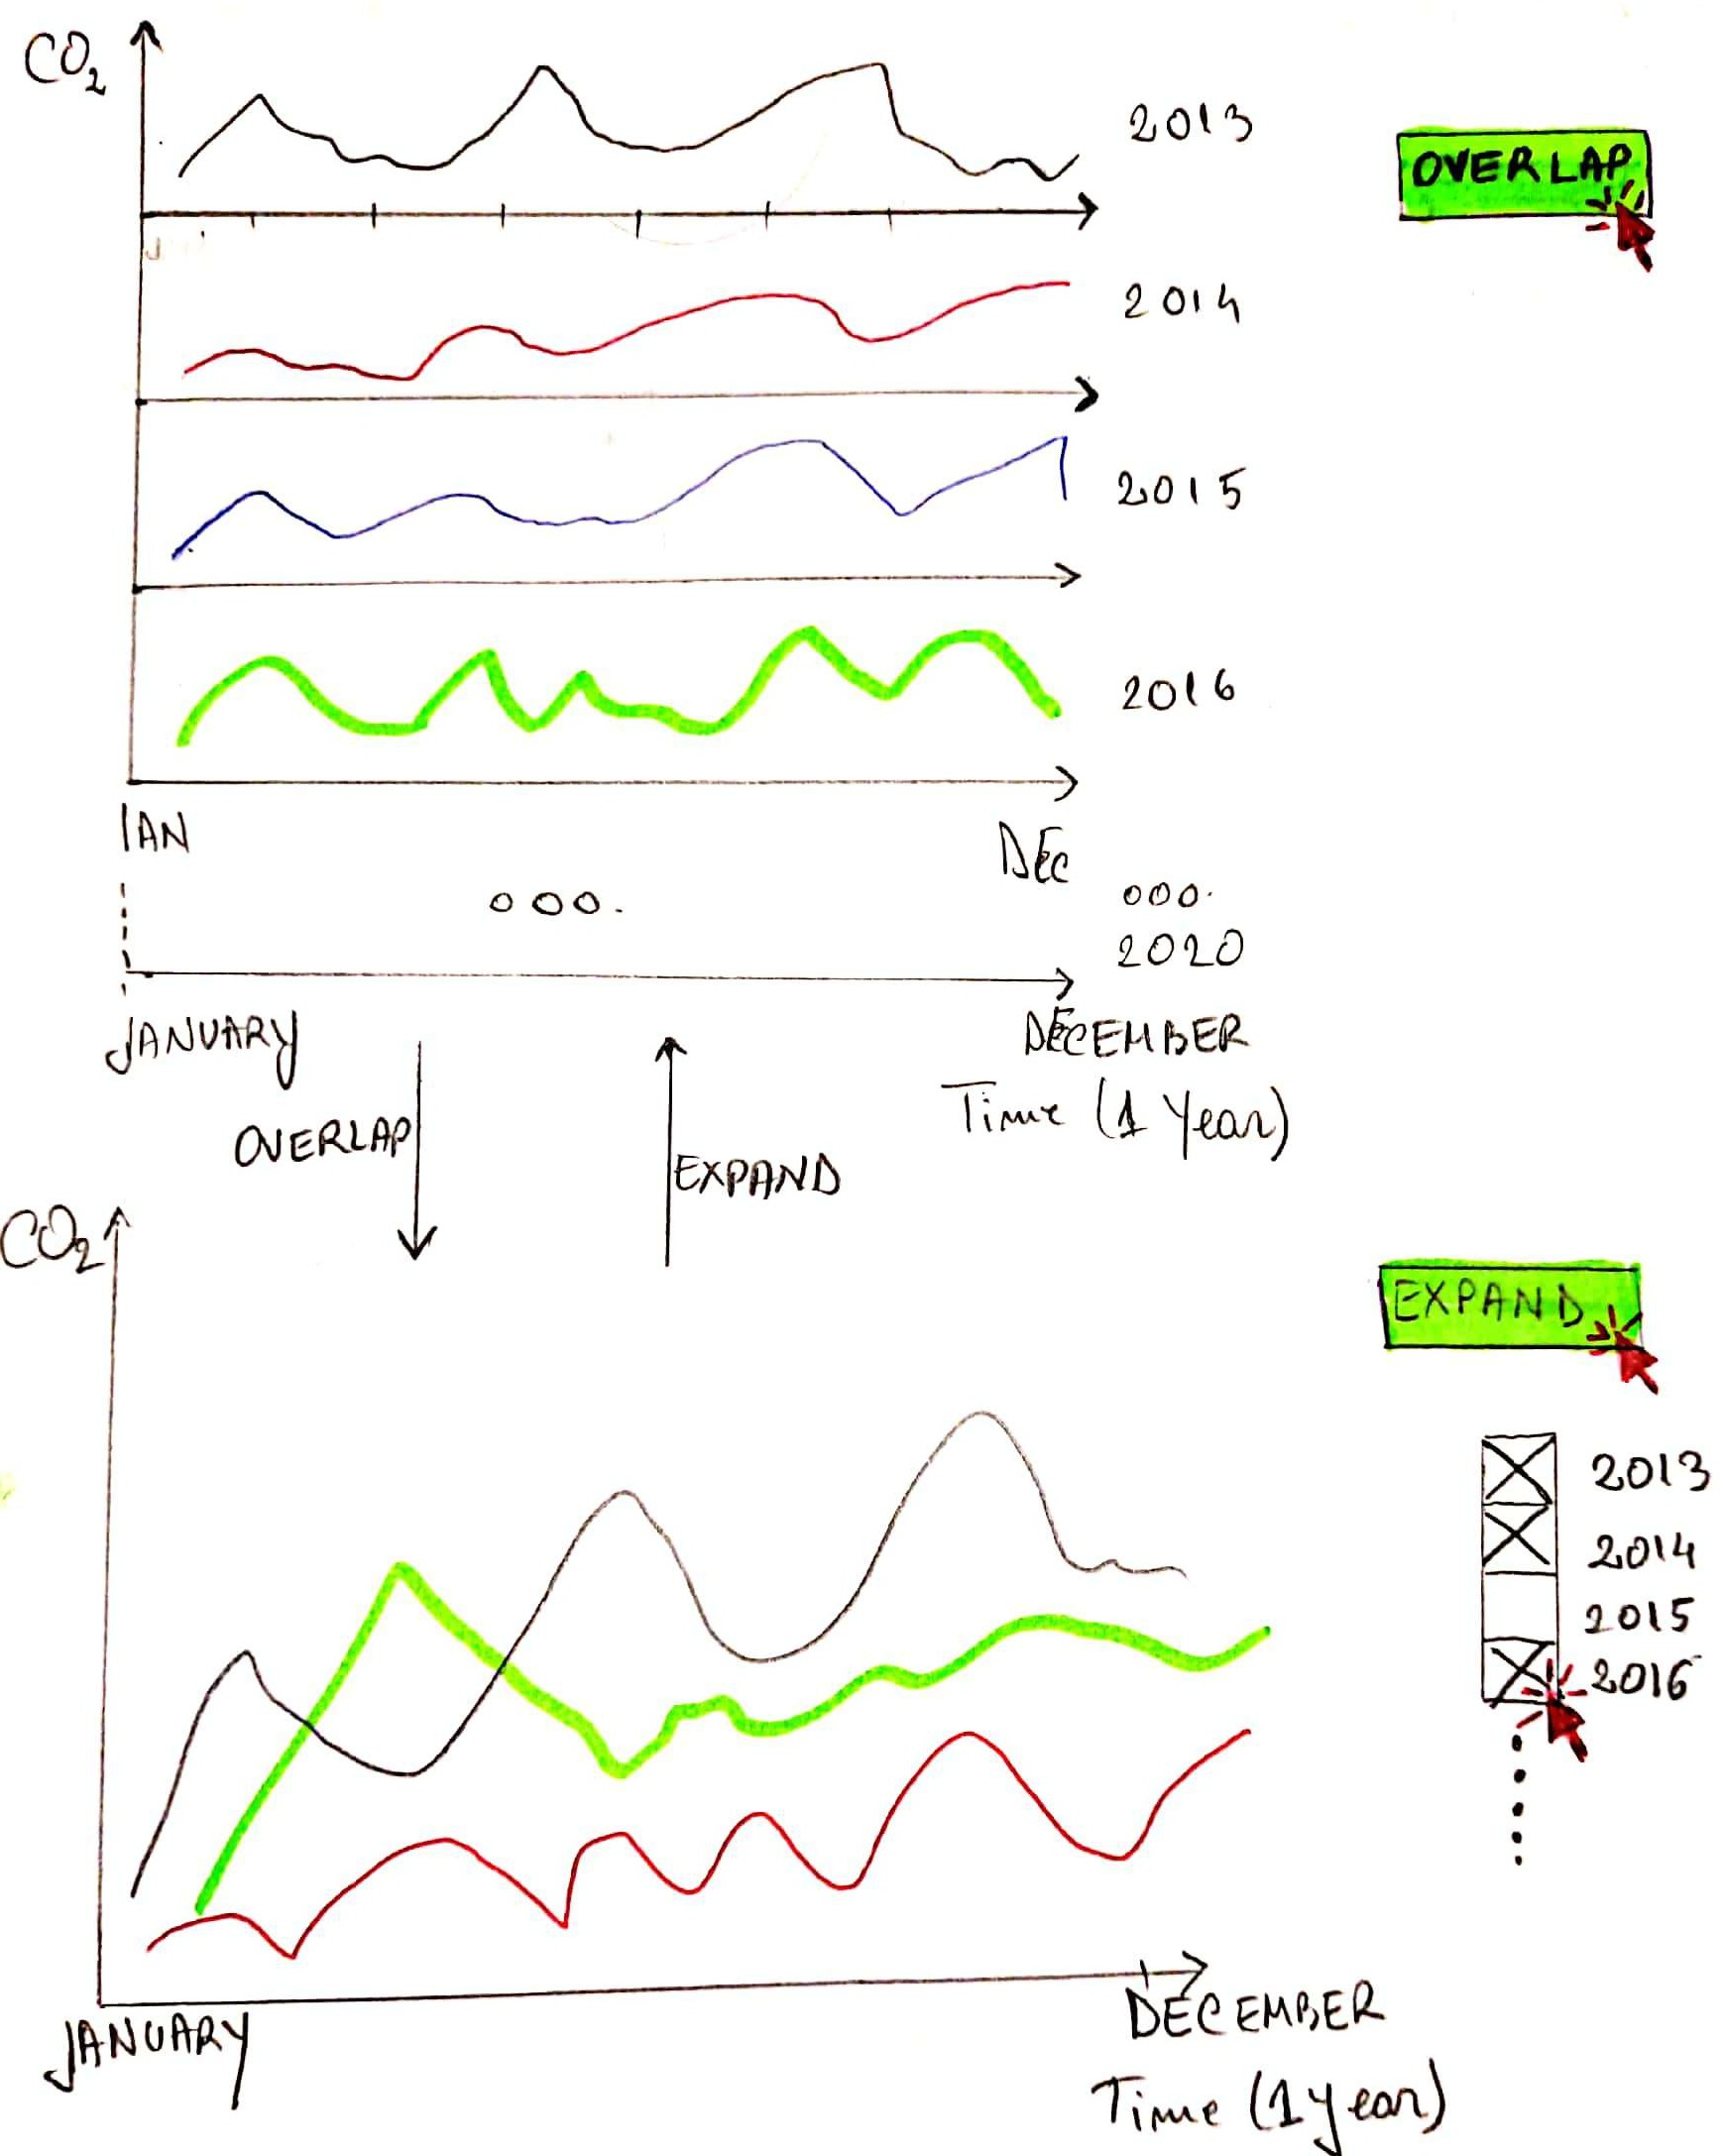
\includegraphics[scale=0.23]{img/1.jpg}
	\caption{CO${_2}$ emissions evolution over time }
	\label{fig:positive_selection}
\end{figure}\

\large{\textbf{Solution 2}}\\
Because I chose to plot the CO${_2}$ variation over one year, and a year can be imagined as a cyclic period of 365 days, we can transform the \textbf{X} axis in a circle, by transforming the $n^{th}$ day from the 1$^{st}$ of January in radians, with the following formula:
\begin{eqnarray}
	\theta = \dfrac{ArcLength * \pi}{L}
\end{eqnarray}

where \textit{L} is the length of the circle given in days(365), and \textit{ArcLength} is the number of days since 1$^{st}$ of January until the date of the mission. Both time and CO${_2}$ are quantities(\textbf{Q}) and the level of CO${_2}$ remains mapped on \textbf{Y} axis. In Table \ref{table2} we can see the visual mapping. 

\begin{table}[h!]
	\begin{center}
		\begin{tabular}{|c | c | c | c || c | c | c | c | c| c| c || c|} 
			\hline
			Name & D & F & D\textquotesingle  & X & Y & Z & T & R & -& [] & CP \\ [0.5ex] 
			\hline\hline
			Time  & Q & $\theta$ & Q &  L &   &   &   &   &   &   &   \\ [0.5ex] 
			\hline
			CO${_2}$  & Q &  &  &  & L  &   &   &   &   &   &   \\ [0.5ex] 
			\hline
			Year  & N &  &  &  &   &   &   & C  &   &   &   \\ [0.5ex] 
			\hline
		\end{tabular}
		\caption{CO${_2}$ emissions evolution  over time}
		\label{table2}
	\end{center}
\end{table}

A visualization would look like in Figure \ref{fig:radians_time}. In this case, the user can only choose which year to be displayed in the visualization and compare it with the average of all years. The list of check boxes in the right side is exclusive, so one choice will uncheck the previous one.
\begin{figure}[H]
	\centering
	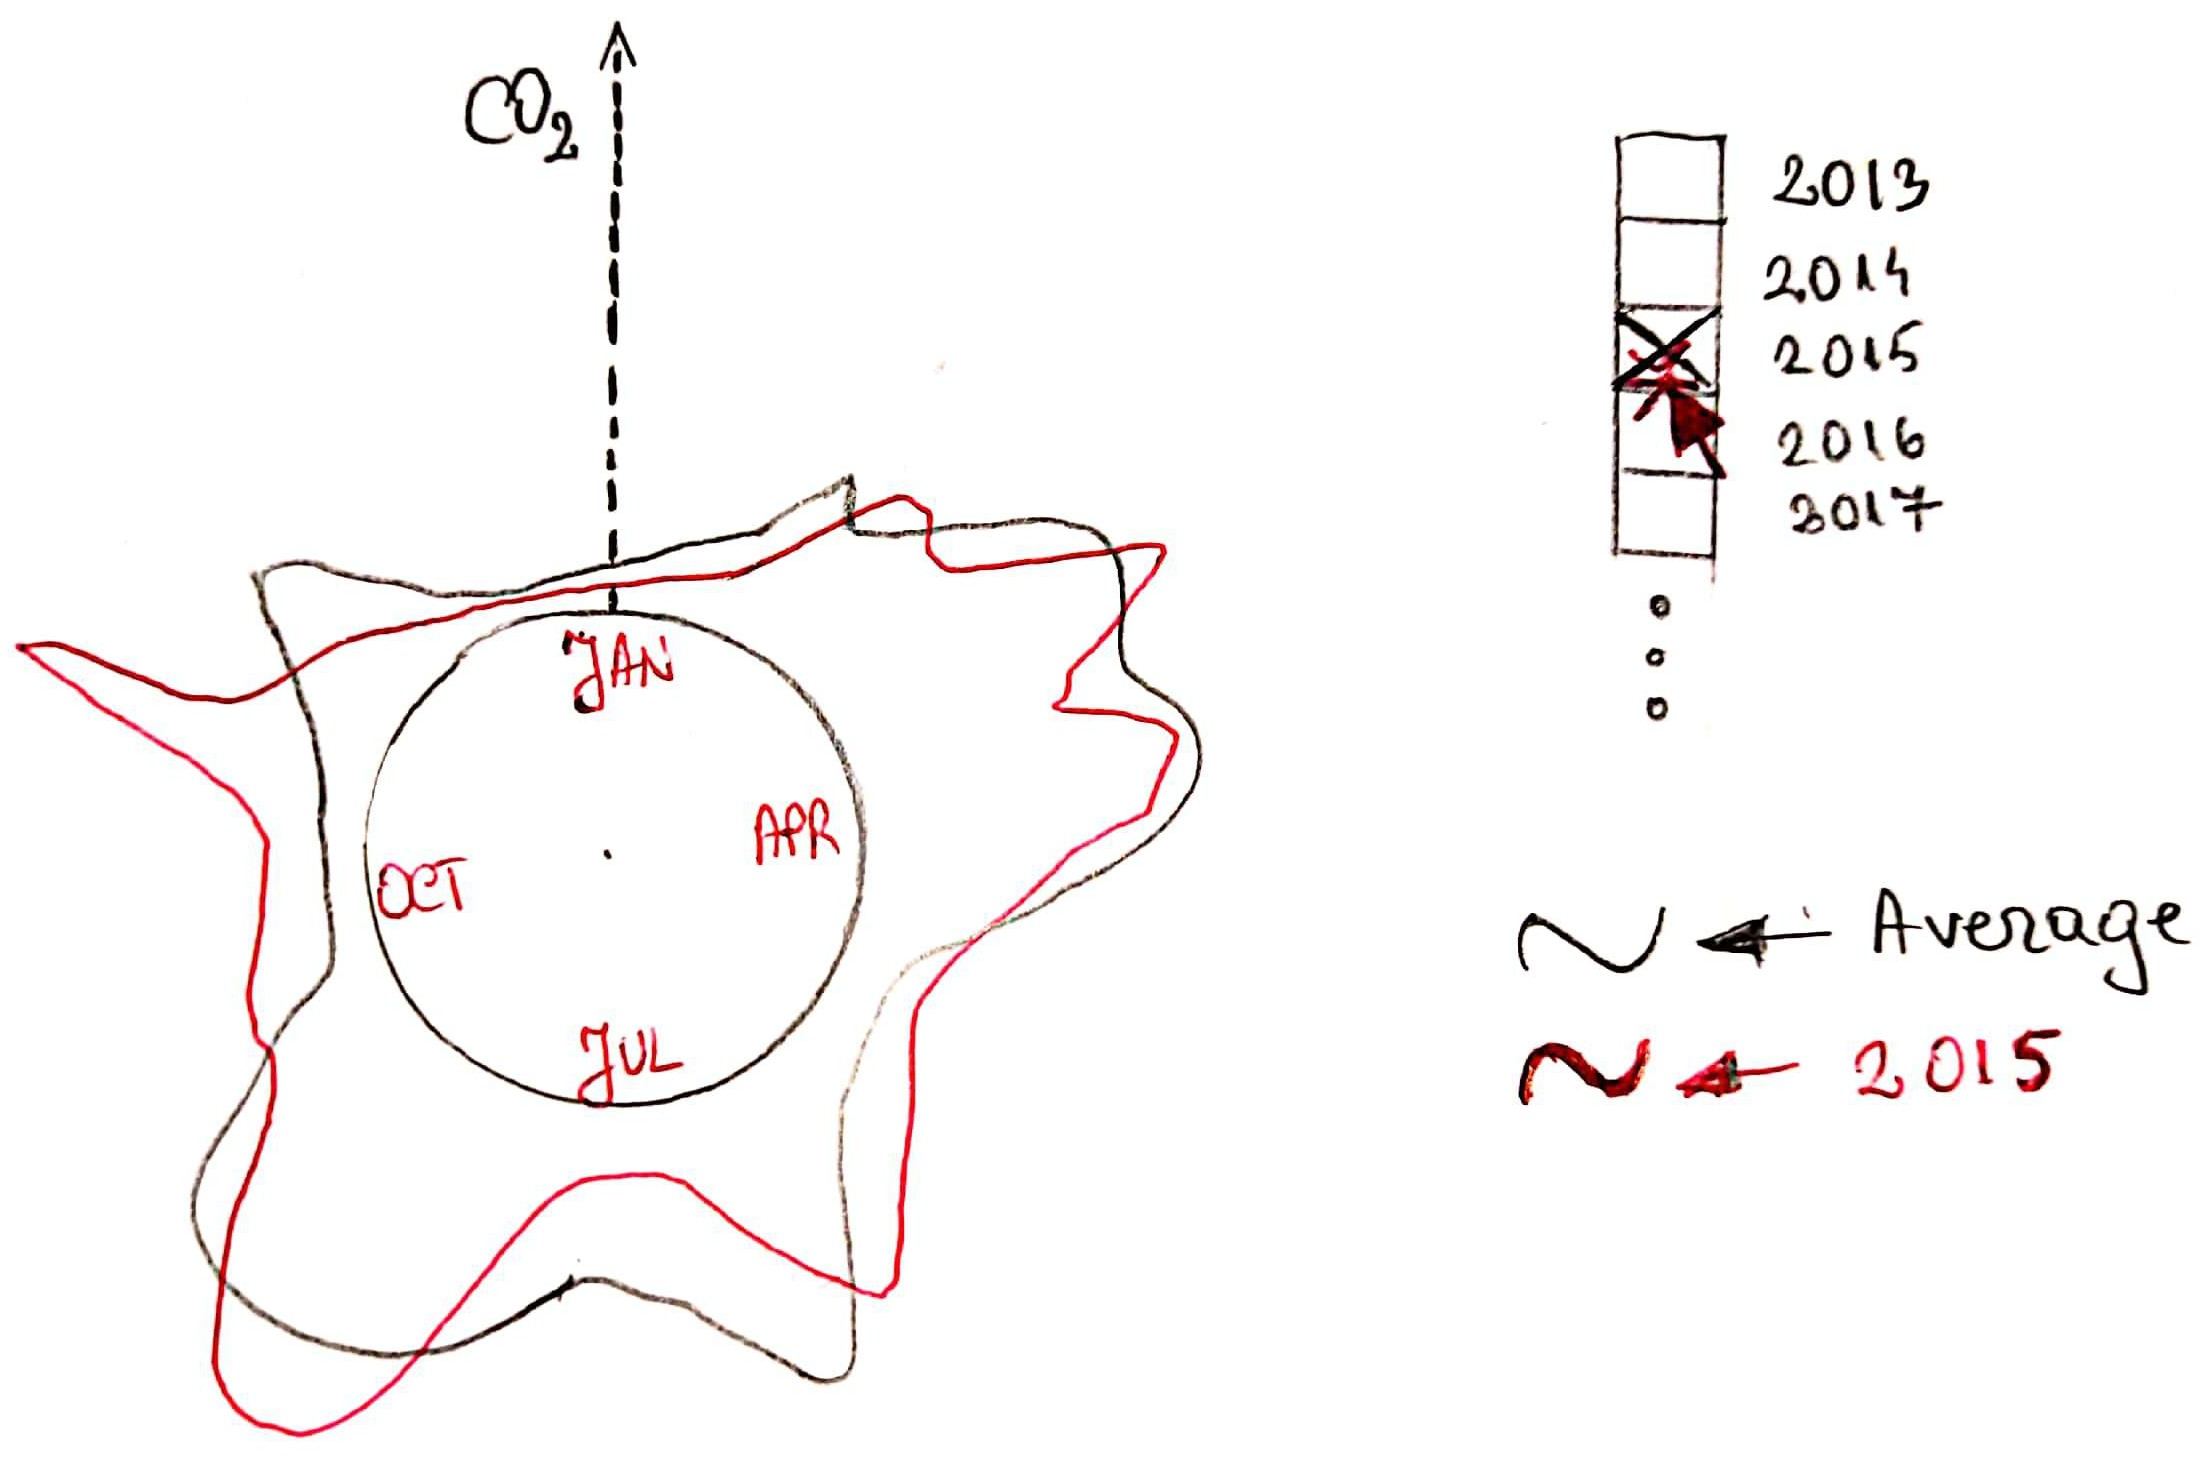
\includegraphics[scale=0.19]{img/3.jpg}
	\caption{CO${_2}$ emissions evolution over time }
	\label{fig:radians_time}
\end{figure}\

\newpage
\section{Where(countries, continents) do most of the users travel? (Distribution of trips to certain places)}
\large{\textbf{Solution 1}}\\
A possible answer to this question would result by providing a list with the first $n$ favorite destinations. To enhance user perception, these can be sorted by the total number of missions and each element of the list is accompanied by the name of the country. The number of missions is a quantity(\textbf{Q}), therefore we can map it on the \textbf{X} axis. Usually, names(of the countries) are nominal values, but I will sort them, thus they become ordinal(\textbf{O}) values. Also, each country can be colored according to its continent, which is a nominal value(\textbf{N}) and encoded as retinal property(\textbf{R}): color(\textbf{C}). For more information of the percentage of the number of missions we can add a Control Processing(\textbf{CP}) property, which will be mapped on the \textbf{X} axis. In Table \ref{table3} we can see the visual mapping.

\begin{table}[h!]
	\begin{center}
		\begin{tabular}{|c | c | c | c || c | c | c | c | c| c| c || c|} 
			\hline
			Name & D & F & D\textquotesingle  & X & Y & Z & T & R & -& [] & CP \\ [0.5ex] 
			\hline\hline
			Nb. of missions & Q &  & Q &  L &   &   &   &   &   &   &   \\ [0.5ex] 
			\hline
			Country  & N & fs & N &  & P  &   &   &   &   &   &   \\ [0.5ex] 
			\hline
			Continent  & N &  & N &  &   &   &   & C  &   &   &   \\ [0.5ex] 
			\hline
			Percentage missions  & Q &  & Q & P &   &   &   &   &   &   & tx  \\ [0.5ex] 
			\hline
			
		\end{tabular}
		\caption{Favorite missions destinations(Sol. 1)}
		\label{table3}
	\end{center}
\end{table}

A sketch is designed in Figure \ref{fig:fav_dest}. What the user needs first to perceive from the image is the order of the countries. Then, for each bar, he will associate the quantity of missions with the country name. I did not encoded the country name as Control Processing(\textbf{CP}) property, since in this case it is more a label of the \textbf{Y} axis. Secondary information would be the grouping of the countries into continents by color of the bars. Notices that there are 7 continents, so Bertin rule on colors is respected.
Depending on the length of the bars, we can use a logarithmic scale. This visualization is not intended to be interactive.
\begin{figure}[H]
	\centering
	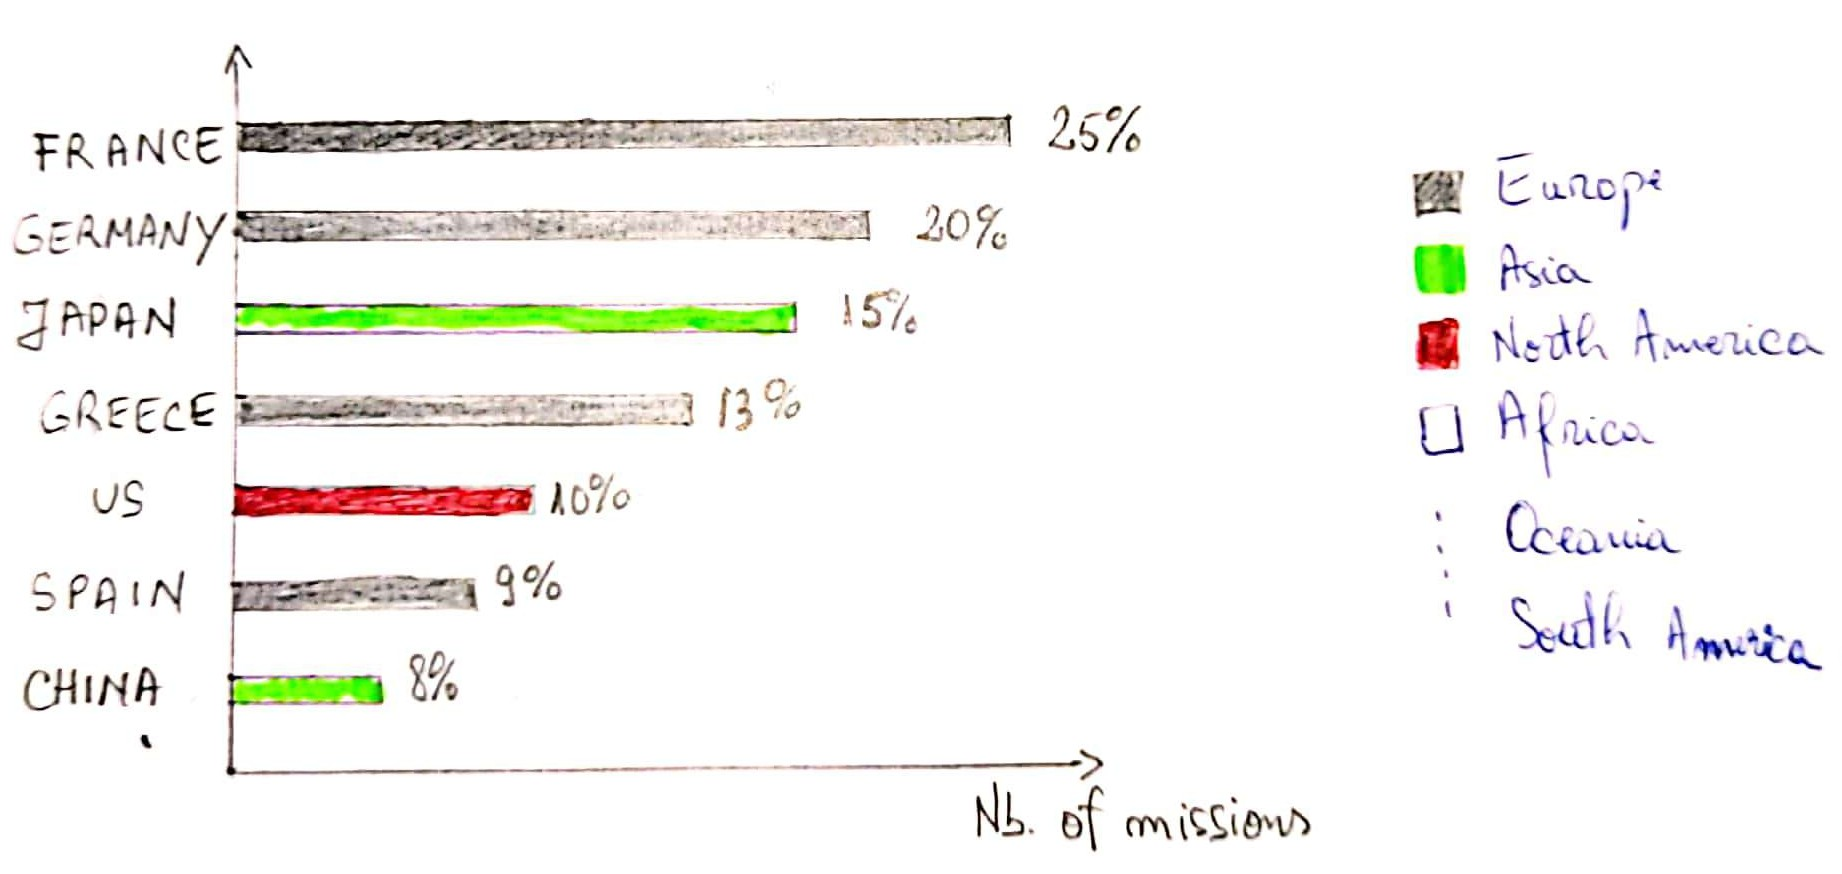
\includegraphics[scale=0.2]{img/4.jpg}
	\caption{Favorite missions destinations(Sol. 1)}
	\label{fig:fav_dest}
\end{figure}\
\newpage

\large{\textbf{Solution 2}}\\
Keeping in mind that we want to show the favorite destinations, we can put a focus on the continents by mapping the number of missions on each continent in a pie-chart. Each slice will have an opening angle($\theta$) which is directly proportional to the length of the arc represented by the number of missions. For this we can use the transformation in radians: Eq.(1), hence the slice for each continent will be a surface(\textbf{S}):

Q$\rightarrow$\textbf{X}:S, \textbf{Y}:S

All the resulted slices will be sorted by the length of the arc(number of missions).


For each country, we calculate the number of missions(\textbf{Q}) and map it as a line on \textbf{Y} axis. 

Q$\rightarrow$\textbf{Y}:L


Countries are nominal(\textbf{N}) values, represented as points on the \textbf{X} axis and sorted inside a continent by the number of missions. Each country is then mapped on the arc which corresponds to the continent to which the country belongs, by using Eq (1). 

Continents are differentiated by the retinal property(\textbf{R}): color and all the countries inside a continent with the same color.

In Table \ref{table4} we can see the visual mapping.



\begin{table}[h!]
	\begin{center}
		\begin{tabular}{|c | c | c | c || c | c | c | c | c| c| c || c|} 
			\hline
			Name & D & F & D\textquotesingle  & X & Y & Z & T & R & -& [] & CP \\ [0.5ex] 
			\hline\hline
			Nb. of missions(continent) & Q &  & Q &  S &  S &   &   &   &   &   &   \\ [0.5ex] 
			\hline
			Nb. of missions(country) & Q &  & Q &   &  L &   &   &   &   &   &   \\ [0.5ex] 
			\hline
			Country  & N & fs, $\theta$ & N & P &   &   &   &   &   &   &   \\ [0.5ex] 
			\hline
			Continent  & N & fs, $\theta$ & N & P &   &   &   & C  &   &   &   \\ [0.5ex] 
			\hline
			
		\end{tabular}
		\caption{Favorite missions destinations(Sol. 2)}
		\label{table4}
	\end{center}
\end{table}
In Figure \ref{fig:fav_dest2} we see the visual representation, which it is not interactive.
\begin{figure}[H]
	\centering
	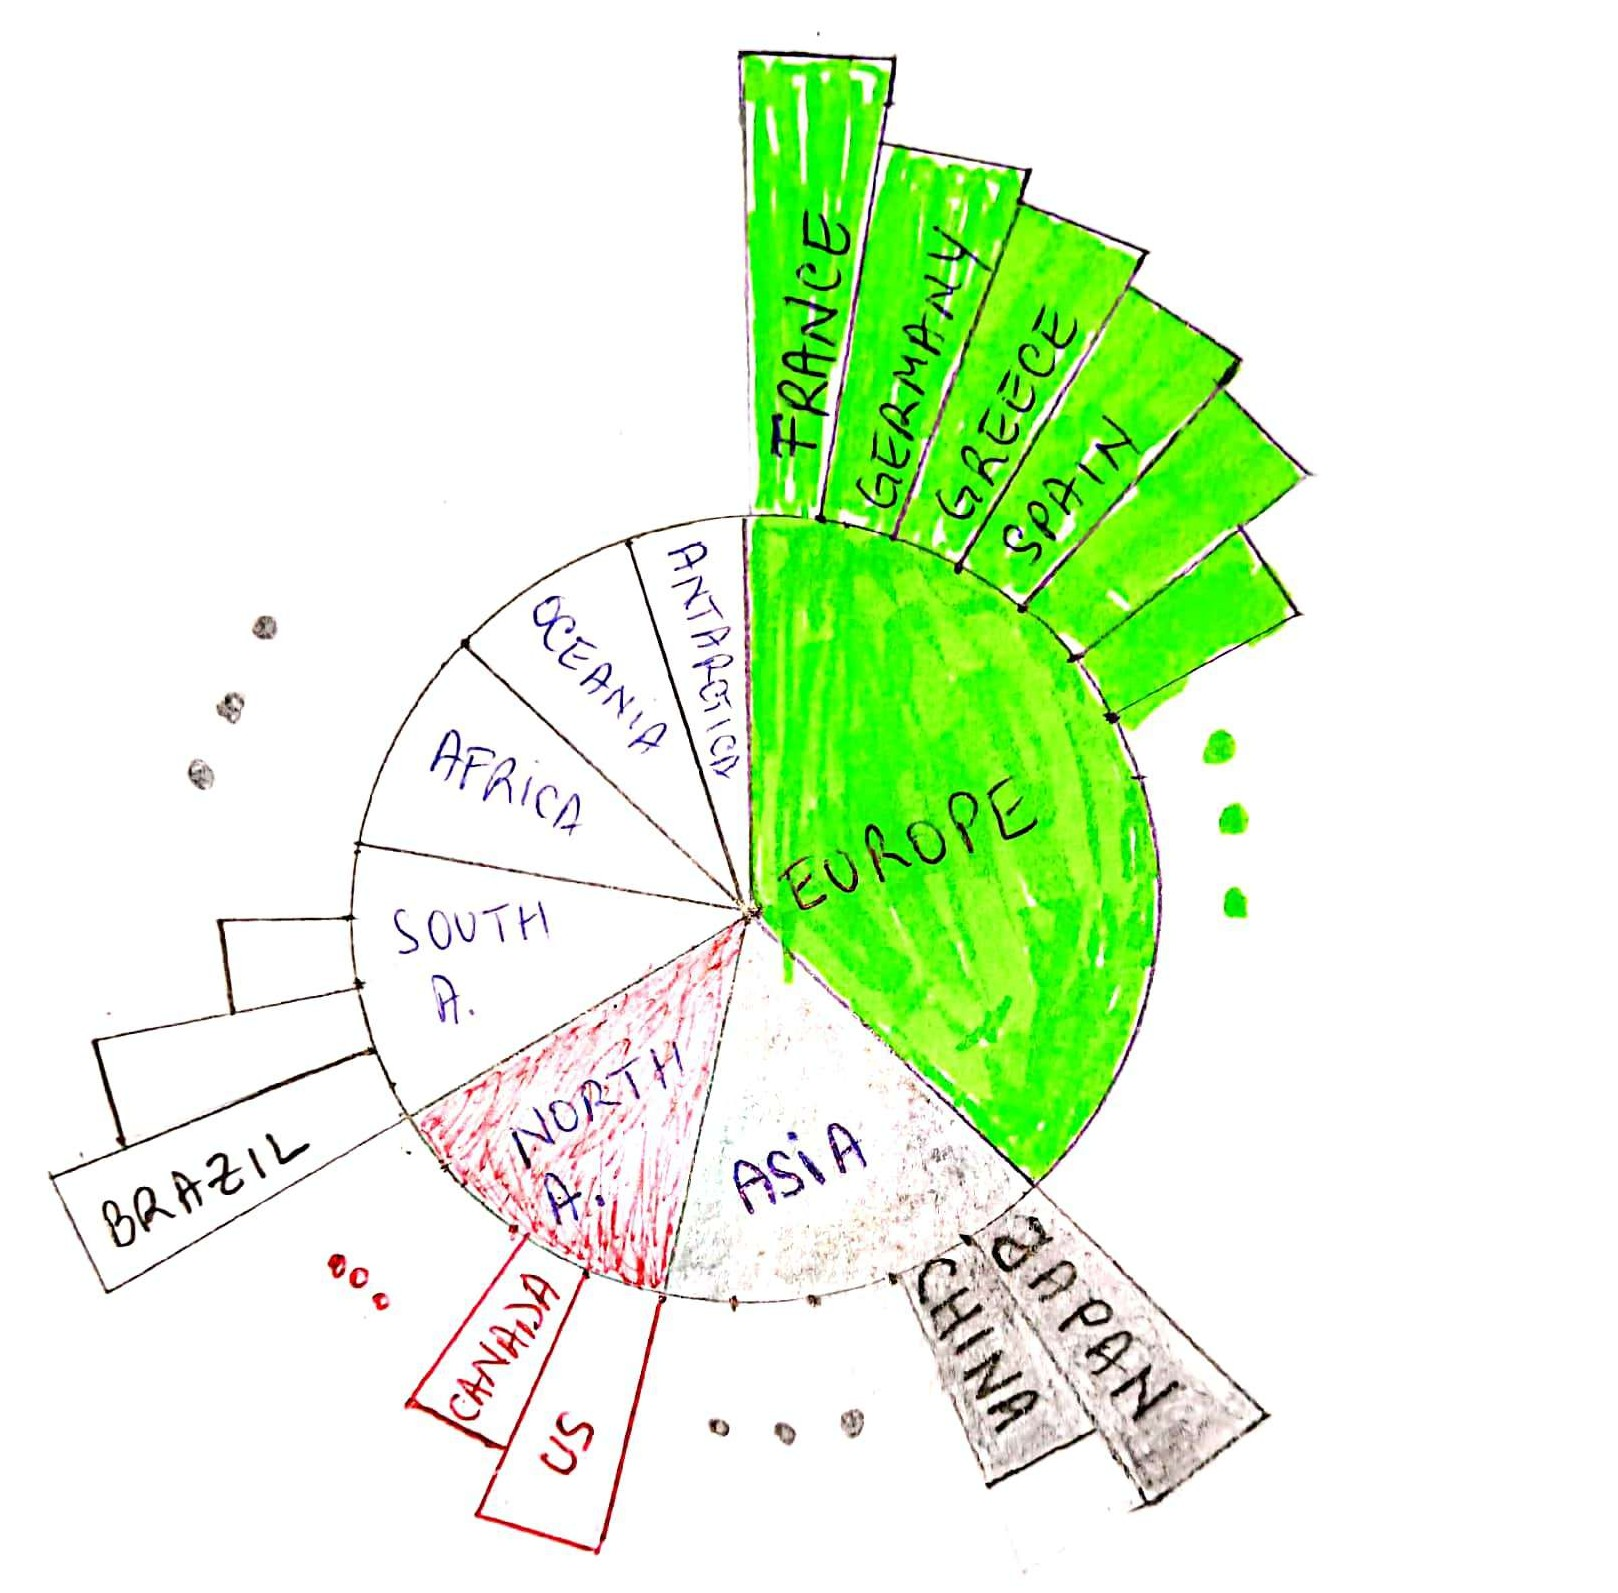
\includegraphics[scale=0.16]{img/5.jpg}
	\caption{Favorite missions destinations(Sol. 2)}
	\label{fig:fav_dest2}
\end{figure}



\large{\textbf{Solution 3}\\}
Another option would be to visualize the number of missions on the world map.

We know the destination country of each mission, therefore we can find out its positional coordinates(long, lat)(we ca use an external dataset which maps countries to their approximately geographical central point).

\textbf{QXlon}$\rightarrow$\textbf{X}:P\\
\textbf{QYlat}$\rightarrow$\textbf{Y}:P

The number of missions can be calculated for a certain time interval, hence a \textbf{slider} can be added to the visualization, to choose the extremities of the interval. We use the retinal property(\textbf{R}) size(\textbf{S}) to encode the number of missions in the interval. Table \ref{table5} shows the visual mapping just described.

\begin{table}[h!]
	\begin{center}
		\begin{tabular}{|c | c | c | c || c | c | c | c | c| c| c || c|} 
			\hline
			Name & D & F & D\textquotesingle  & X & Y & Z & T & R & -& [] & CP \\ [0.5ex] 
			\hline\hline
			Long.  & QX lon &  & QX lon &  P &   &   &   &   &   &   &   \\ [0.5ex] 
			\hline
			Lat  & QY lat &  & QY lat &  & P  &   &   &   &   &   &   \\ [0.5ex] 
			\hline
			Nb. of missions(country)  & Q & sl & Q &  &   &   &   & S  &   &   &   \\ [0.5ex] 
			\hline
		\end{tabular}
		\caption{Visual mapping: favorite missions destinations(Sol. 3)}
		\label{table5}
	\end{center}
\end{table}

In Figure \ref{fig:fav_dest_world} we can see how a visualization would look like for the previous visual mapping. The initial map shows all the continents with a red circle on each country, with the diameter directly proportional to the number of missions to that destination. Using the mouse cursor, a rectangle region can be selected to be maximized. Selecting the European continent, the result it's shown in Figure \ref{fig:fav_dest_europe}.

\begin{figure}[H]
	\centering
	\tcbox{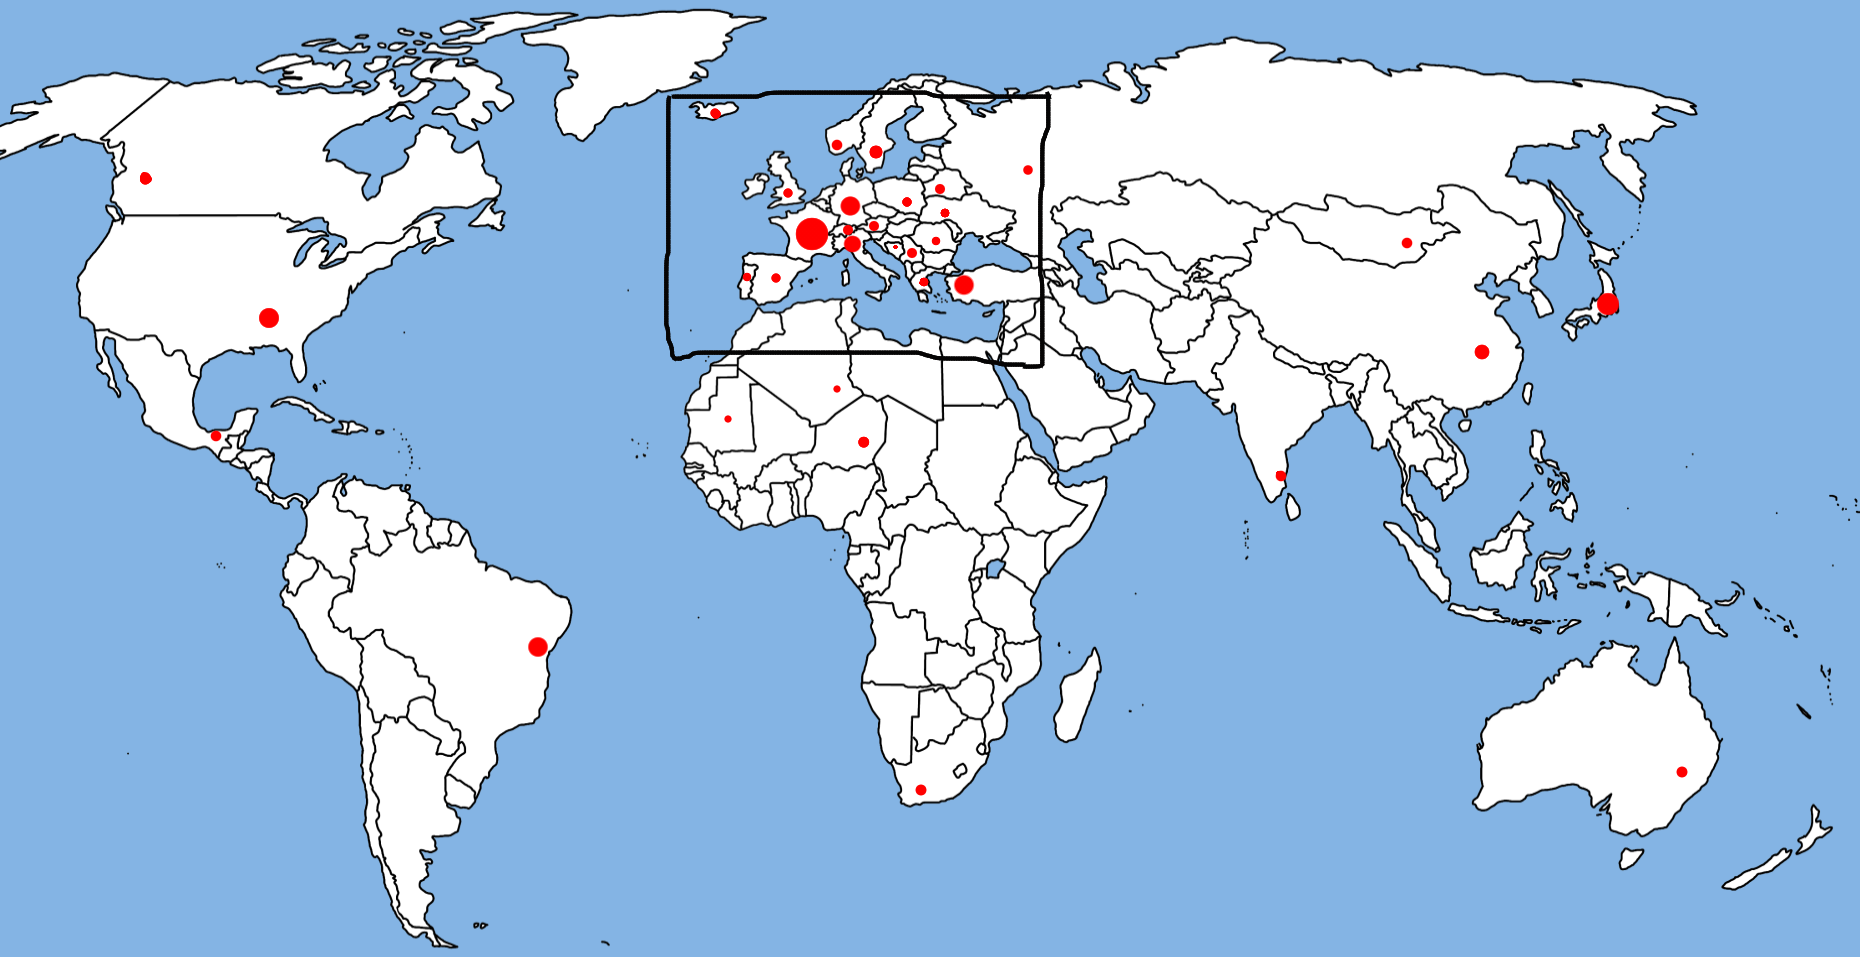
\includegraphics[scale=0.18]{img/5_5.png}}
	\caption{Favorite missions destinations(Sol. 3) - Fictive data}
	\label{fig:fav_dest_world}
\end{figure}

\begin{figure}[H]
	\centering
	\tcbox{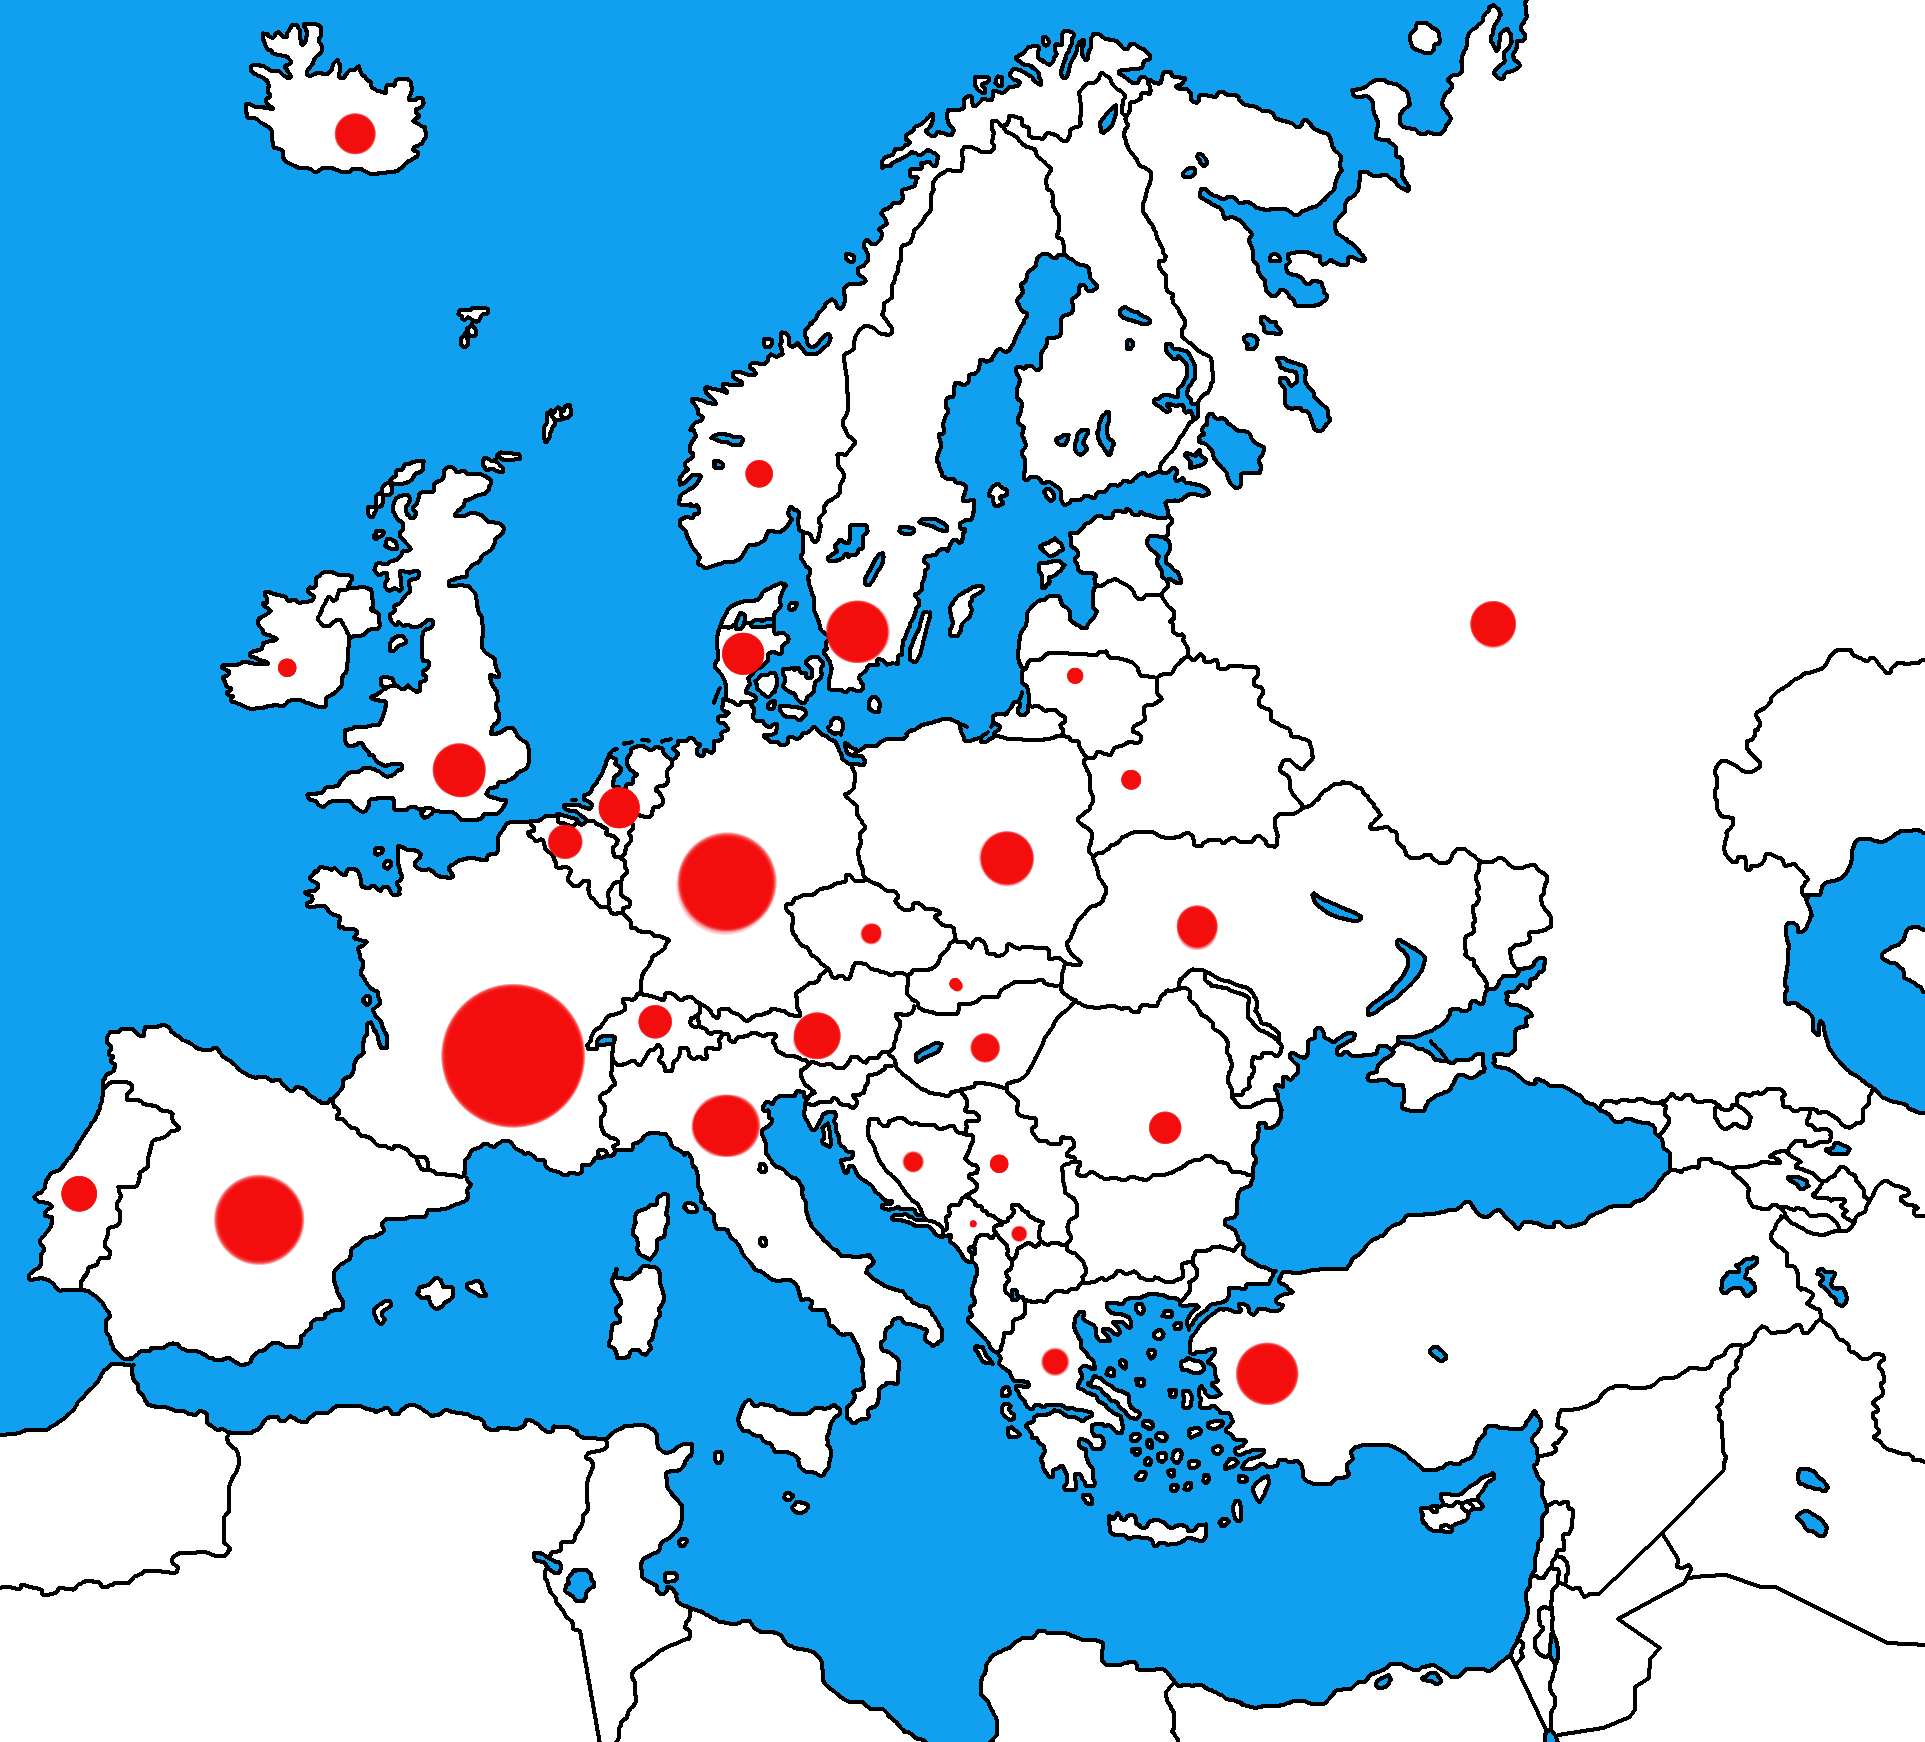
\includegraphics[scale=0.18]{img/6.png}}
	\caption{Favorite missions destinations(Sol. 3) - Fictive data}
	\label{fig:fav_dest_europe}
\end{figure}

The visualization has a slider attached that is represented in Figure \ref{fig:fav_dest_glider}. For the plot, it will be counted only the missions that started in the desired interval. The user can change the extremities of the interval by moving the red triangles, or can slide it, in this way providing a continuity effect of the evolution of the number of missions in the range.\\


\begin{figure}[H]
	\centering
	\tcbox{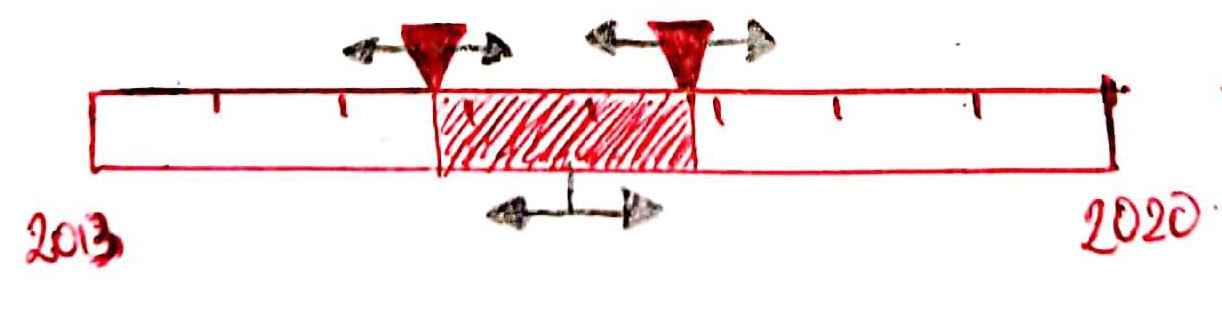
\includegraphics[scale=0.2]{img/7.jpg}}
	\caption{Date glider}
	\label{fig:fav_dest_glider}
\end{figure}



\textbf{\Large{B. Focusing on subsets}}\\
\section{Which person, house, region, rank, title, institution pollutes the most?}

Starting from the sample visualization provided in the project, of the CO${_2}$ distribution over people, it is interesting to observe if any of the subsets mentioned in the question is predisposed to higher/lower levels of CO${_2}$ emissions for any of its components.

An example would be to see if people who produce small amounts of CO${_2}$ emissions have lower ranks, or maybe they are part of a certain institutions, or they have a prestigious title.

With this in mind, and considering that a person may be considered a subset of dimension 1, we can design a visualization that shows statistics on all subsets of our dataset and possible correlations between them.

A key point in selecting people who produce large/small amounts of CO${_2}$, is to add a slider in the provided visualization, to take into consideration only a range of users. On the \textbf{X} axis, users are mapped as quantity(\textbf{Q}), and on the \textbf{Y} axis, the volume of CO${_2}$ is mapped also as quantity(\textbf{Q}). We want to have the users sorted by the quantity of CO${_2}$ produced, so we apply a sort function, then a slider in order to select the users from a certain interval. In Table \ref{table6} we have the visual mapping.

We can interact with the visualization by moving the interval extremities with the cursor. The surface in the interval can be represented with a color different than the one outside the interval.
 
 \begin{table}[h!]
 	\begin{center}
 		\begin{tabular}{|c | c | c | c || c | c | c | c | c| c| c || c|} 
 			\hline
 			Name & D & F & D\textquotesingle  & X & Y & Z & T & R & -& [] & CP \\ [0.5ex] 
 			\hline\hline
 			Users  & Q & s,sl & O &  S &   &   &   &   &   &   &   \\ [0.5ex] 
 			\hline
 			CO${_2}$  & Q &  & Q &  & S  &   &   &   &   &   &   \\ [0.5ex] 
 			\hline
 		\end{tabular}
 		\caption{Visual mapping: CO${_2}$ over users(vis.1 in Figure \ref{fig:subsets} )}
 		\label{table6}
 	\end{center}
 \end{table}

For the: distribution of CO${_2}$ over ranks, titles, regions and institutions, the visualizations are similar. On the \textbf{X} axis, we map the emissions of CO${_2}$ as quantity\textbf{(Q)} and on the \textbf{Y} axis we map the categories mentioned before as points(the order is not taken into account). I will provide the visual mapping only for the rank distribution in Table \ref{table7}, because the others(vis. 4, 5, 6 from Figure \ref{fig:subsets}) are almost identical. It is important to mention that for each title, rank, etc., we compute the average of the CO${_2}$ produced by the users inside each group.

\begin{table}[h!]
	\begin{center}
		\begin{tabular}{|c | c | c | c || c | c | c | c | c| c| c || c|} 
			\hline
			Name & D & F & D\textquotesingle  & X & Y & Z & T & R & -& [] & CP \\ [0.5ex] 
			\hline\hline
			CO${_2}$ & Q &  & Q &  L &   &   &   &   &   &   &   \\ [0.5ex] 
			\hline
			Rank  & Q &  & Q &  & P  &   &   &   &   &   &   \\ [0.5ex] 
			\hline
			
		\end{tabular}
		\caption{CO${_2}$ distribution over ranks(vis.2 in Figure \ref{fig:subsets} )}
		\label{table7}
	\end{center}
\end{table}

Visualization 2 from Figure \ref{fig:subsets} could provide some interesting insight about the emissions of CO${_2}$ inside a house. It is like vis. 1, but instead of having the users on the \textbf{X} axis, we map the houses, and on the \textbf{Y} axis, the average CO${_2}$ quantity produced inside a house, then all the values are sorted, resulting almost an exponential curve. We consider that all the houses are "vertical cylinders" of equal width. By moving the slider extremities in the vis. 1, we keep inside a house just a number of users equal with those that are in the slider range interval. Therefore, some regions in the houses distribution will become whiter in color, if we consider that inside a house, we eliminate randomly the users from a house, its color going from black to gray (if the initial color is black). In Figure \ref{fig:subsets}, vis.2, we can see such an effect.

\begin{figure}[H]
	\centering
	\tcbox{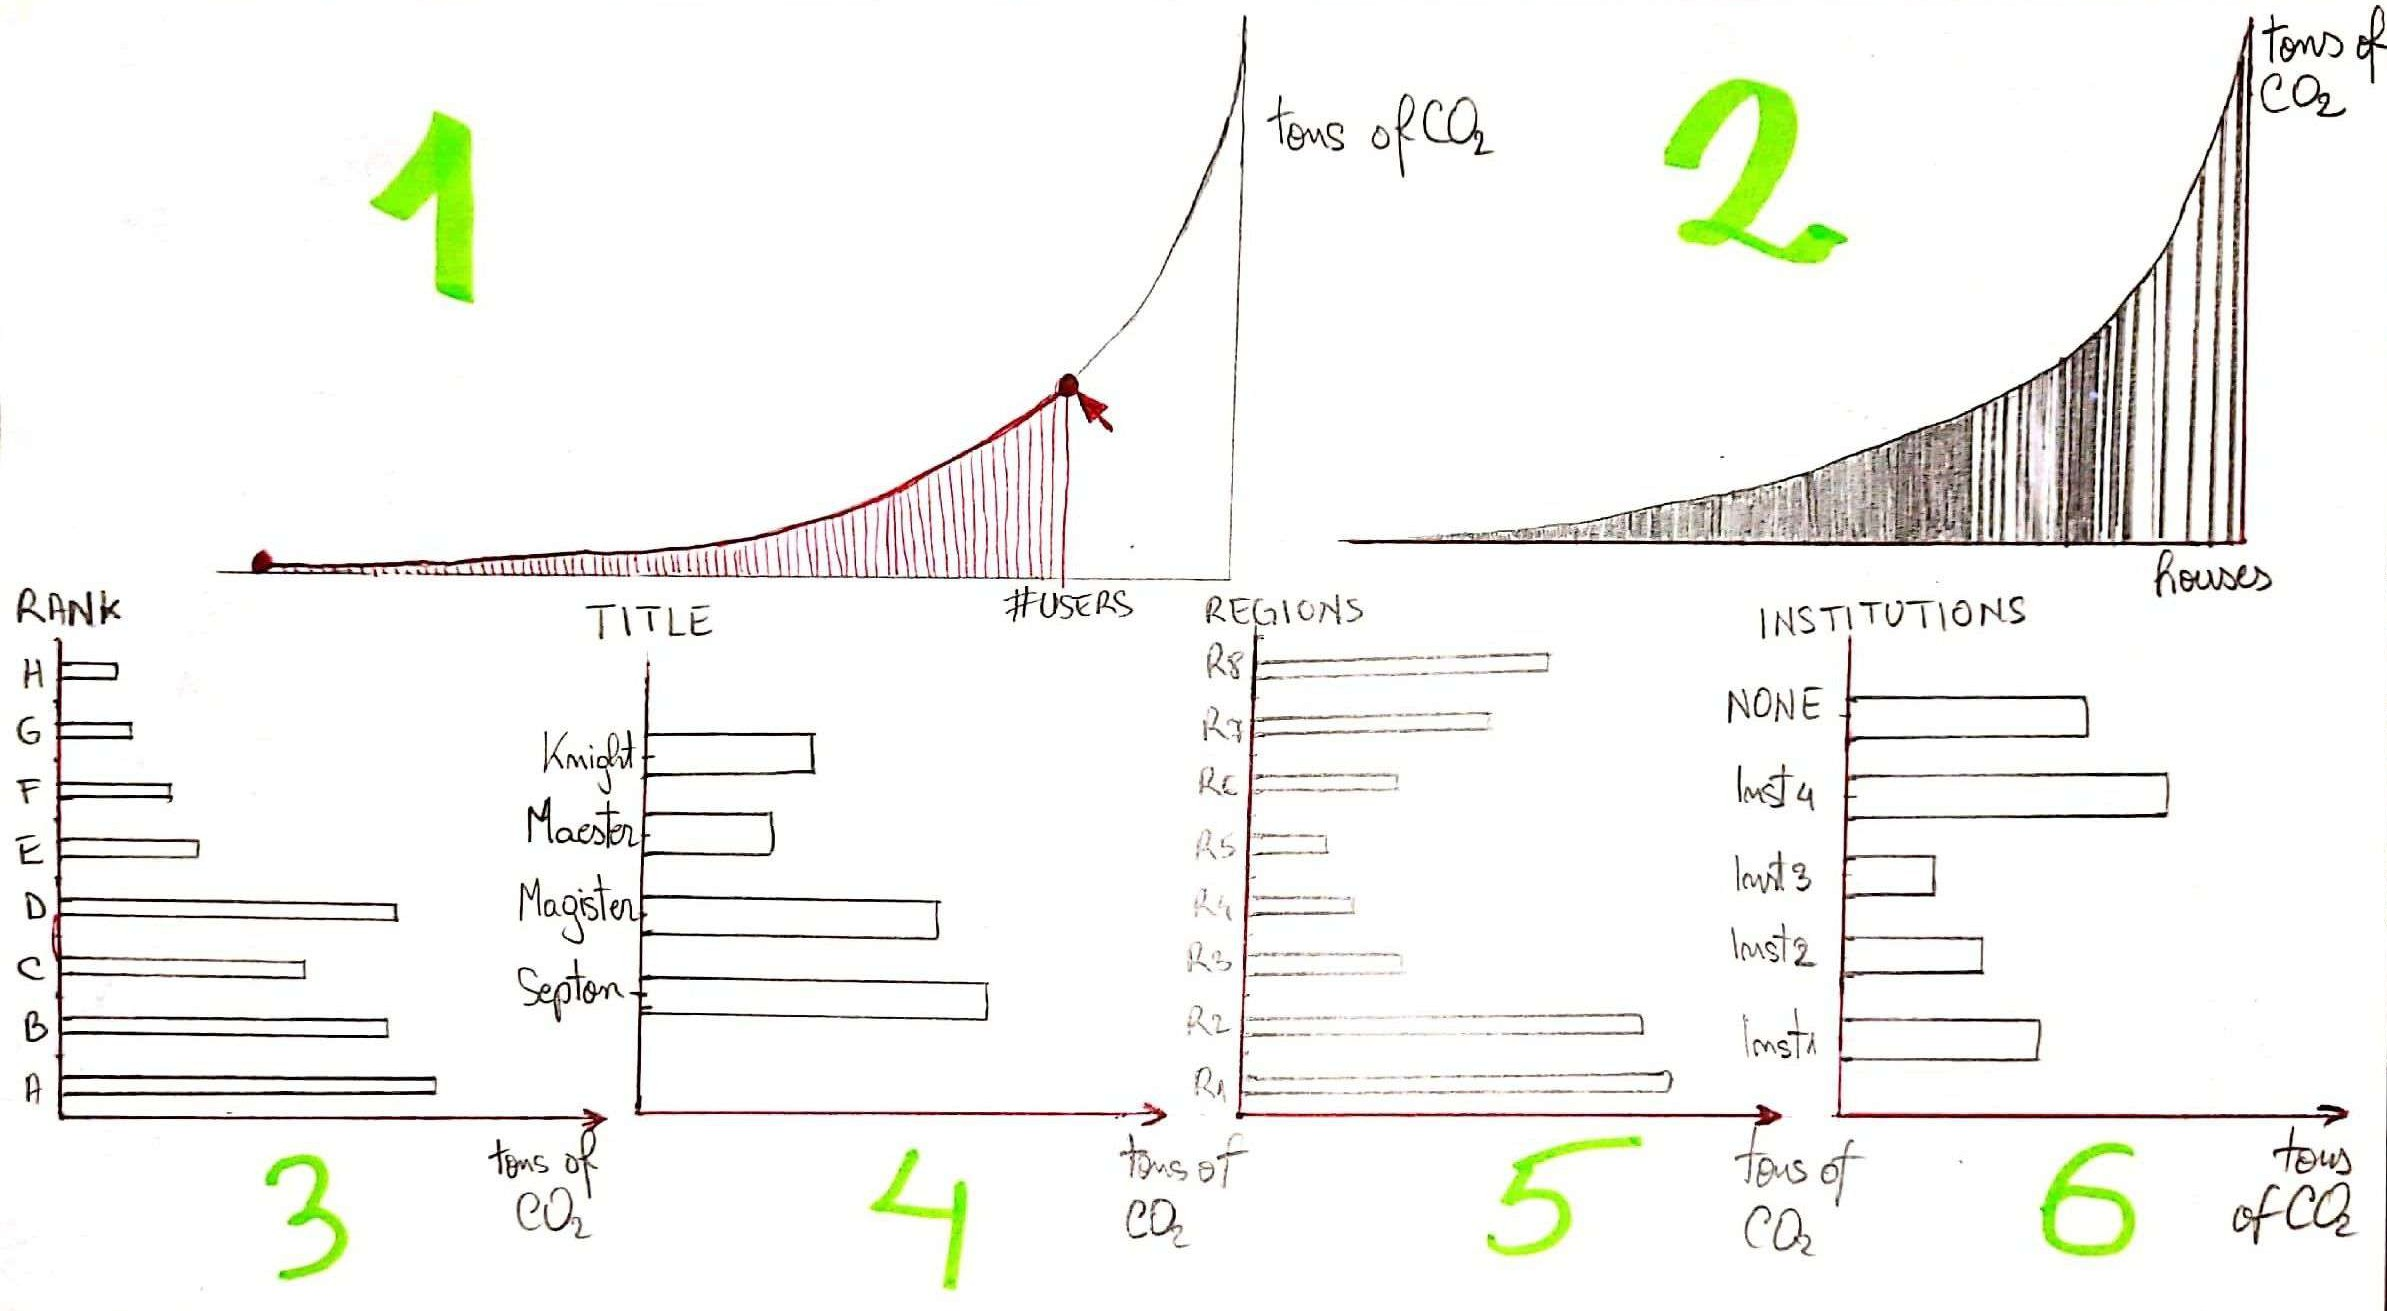
\includegraphics[scale=0.18]{img/8_5.jpg}}
	\caption{CO${_2}$ - subsets statistics}
	\label{fig:subsets}
\end{figure}


%
%\section{How much CO${_2}$ emissions are produced to go to certain places?(Distribution of CO$_2$ over the countries)}
%Solution\\
%This question is very similar to the previous one, this time instead of counting how many missions take place in a country, we count the CO${_2}$ emissions produced to go there, my multiplying the CO${_2}$ quantity released per km with the distance to destination and the number of missions to that place.
%
%We can map the CO${_2}$ emissions on the \textbf{X} axis, since it is a quantity(\textbf{Q}) and on the \textbf{Y} axis we can map the countries in descending order with horizontal bars, showing the amount of CO${_2}$.
%
%The continent is mapped as color and the percentage of emissions for a country as text, thus we will have the visual mapping from Table \ref{table_CO2}.
%
%\begin{table}[h!]
%	\begin{center}
%		\begin{tabular}{|c | c | c | c || c | c | c | c | c| c| c || c|} 
%			\hline
%			Name & D & F & D\textquotesingle  & X & Y & Z & T & R & -& [] & CP \\ [0.5ex] 
%			\hline\hline
%			CO${_2}$ & Q &  & Q &  L &   &   &   &   &   &   &   \\ [0.5ex] 
%			\hline
%			Country  & N & fs & N &  & P  &   &   &   &   &   &   \\ [0.5ex] 
%			\hline
%			Continent  & N &  & N &  &   &   &   & C  &   &   &   \\ [0.5ex] 
%			\hline
%			Percentage emissions  & Q &  & Q & P &   &   &   &   &   &   & tx  \\ [0.5ex] 
%			\hline			
%		\end{tabular}
%		\caption{CO${_2}$ emissions over countries}
%		\label{table_CO2}
%	\end{center}
%\end{table}
%
%A sketch would look like the one from Figure \ref{fig:fav_dest}, therefore we can add on it a transition button, to switch between the two distributions.

%	\item Is the mission mode correlated with the distance/country?
%	\item What are the CO${_2}$ emissions for a certain rank/title/house?
%	\item Which rank/title/house spent the most time in missions?
%	\item Which rank/title/house traveled the longest distance?
%	\item Which rank/title/house completed most of the missions?


\newpage

\bibliographystyle{plain}
\bibliography{bibliography}


\end{document}
